%%=============================================================================
%% Voorgeschiedenis Universiteit Gent
%%=============================================================================

\chapter{Voorgeschiedenis netwerk van Universiteit Gent}%
\label{ch:voorgeschiedenis}

% TODO: Inleiding voorgeschiedenis
Dit hoofdstuk zal eerst een overzicht geven van de huidige werking voor netwerkbeheerders binnen \acrshort{ugent}.
Daarna wordt beschreven welke stappen reeds zijn ondernomen om deze werking aan te passen om \acrlong{eip} te implementeren.

\section{Huidige werking Universiteit Gent}
\textcolor{purple}{Bij de aanvang van de bachelorproef is het netwerk van \acrshort{ugent} nog volledig beheerd via subnetbestanden. Binnen het netwerkteam van UGent werd een standaard bepaald en toegepast voor het nummeren en klasseren van subnetten, de zogenaamde ARWA-standaard (naar oud-werknemer ARsene WAuters). Dankzij scripts worden deze subnetbestanden uitgelezen en wordt alle nodige informatie doorgegeven aan o.a. de \acrshort{dns}- en \acrshort{dhcp}-servers. Daarnaast genereren deze scripts ook \acrfull{acl}-regels die dan via update-scripts op de routers kunnen geplaatst worden.}

\subsection{Subnetbestanden}
\label{subnetbestanden}
\textcolor{purple}{Op basis van ARWA-standaard krijgt elk subnetbestand een naam: “subnet” + subnet klasse (A/B/C/D/G/I/N/P/T/V/W) + subnetnummer (laatste 2 octetten van het netwerkadres). Elk subnetwerk binnen \acrshort{ugent} komt overeen met een of meerdere subnetbestanden, afhankelijk van de grootte van het subnetwerk. Een subnetwerk dat meer dan 254 beschikbare \acrshort{ip}-adressen bevat, komt overeen met meerdere, opeenvolgende, subnetbestanden. Indien een subnetwerk minder dan 254 hostadressen bevat, bijvoorbeeld 126, zal dit subnetbestand ook maar 126 hosts bevatten.
Zo stelt bijvoorbeeld het subnetbestand “subnetB147.000” het subnet 157.193.147.0/24 voor, en subnetbestand “subnetB050.128” het subnet 157.193.50.128/25. Deze ongeëncrypteerde tekstbestanden stellen elk een deel , of een volledig subnet voor.}
\begin{itemize}
    \item Header: Elk bestand begint met een “header” waarin belangrijke metadata beschreven staat over het netwerk, een voorbeeld is terug te vinden in figuur \ref{fig:header}. Belangrijk hier nog bij op te merken is dat subnet plaats gebruik maakt van de gebouwcodes die \acrshort{ugent} gebruikt. Daarnaast staan de optionele S-lijnen voor \acrfull{acl}-lijnen (beveiligingregels die toegang geven of weigeren voor een of meerdere subnetten of hosts) om extra toegang te voorzien aan het netwerk. 
    \item Hosts: Afhankelijk van de grootte van het subnet kunnen er tot 254 hosts beschreven staan in het bestand. Elk hostadres, of die nu reeds bezet is of niet, staat beschreven in het subnetbestand. Hierbij krijg je dan een opsomming van alle informatie, waarbij elk informatieveld vooraf wordt gegaan door de relevante code. Een hostadres dat niet bezet is bevat, naast het nummer (die de laatste octet weergeeft van het \acrshort{ip}-adres), enkel lege velden zoals te zien in \ref{fig:legehost}. Naast de data voor elke host kan een netwerkbeheerder ook extra lijnen toevoegen voor \acrshort{dns} A en CNAME resource records “AA: en CA:”, het openzetten van de beveiliging richting de host met “S: en SI:” en ook extra mailinformatie “MD:”. Een voorbeeld van een bezette host is figuur \ref{fig:bezettehost}.
\end{itemize}

% TODO: 30.01 uit subnet plaats halen
\begin{figure}[H]
    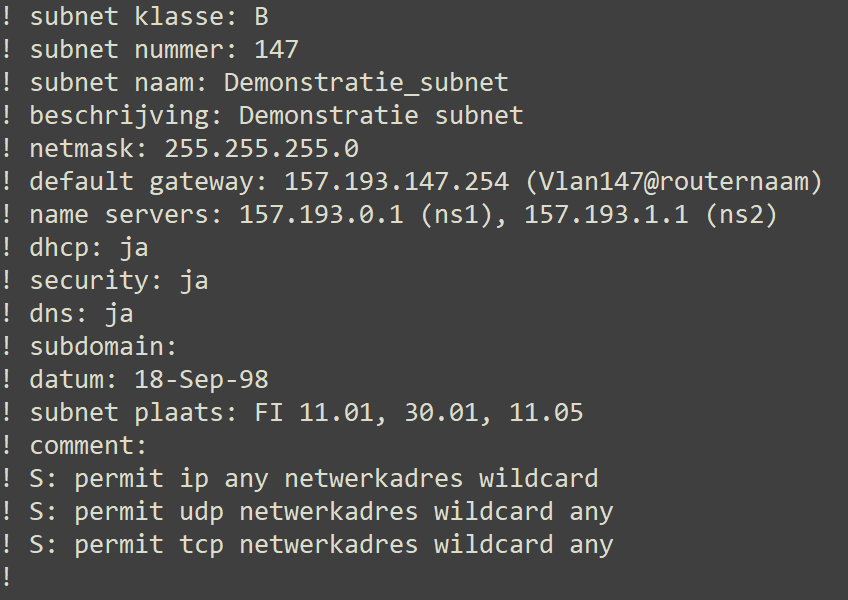
\includegraphics[height=7cm]{header.png}
    \caption{Header in subnetbestanden}
    \label{fig:header}
\end{figure}

% TODO: Hostnaam aanpassen voorbeeld
\begin{figure}[H]
    \subfloat[\acrshort{ip} reservatie voor het eerste adres in het subnet]{%
        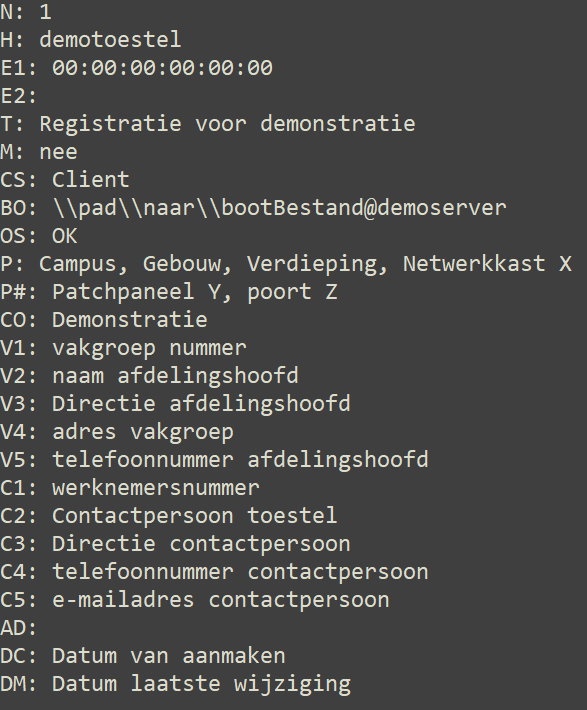
\includegraphics[height=0.4\textheight]{host.png}\label{fig:bezettehost}}
    \hspace*{\fill}
    \subfloat[Derde adres in het subnet is vrij om in te nemen]{%
        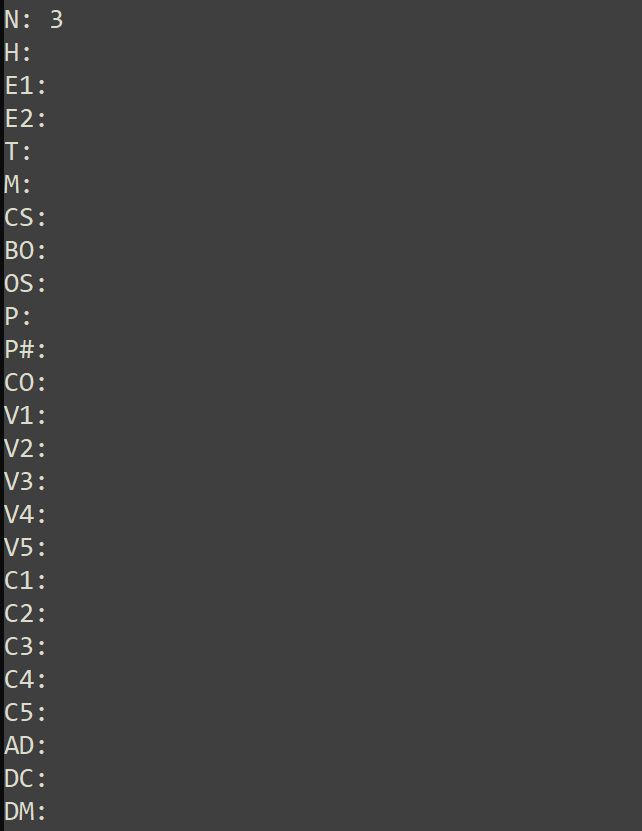
\includegraphics[height=0.4\textheight]{legeHost.png}\label{fig:legehost}}
    \caption{\acrshort{ip} reservatie en lege host entry in subnetbestanden}
    \label{fig:host}
\end{figure}



%\begin{figure}[h!]
%    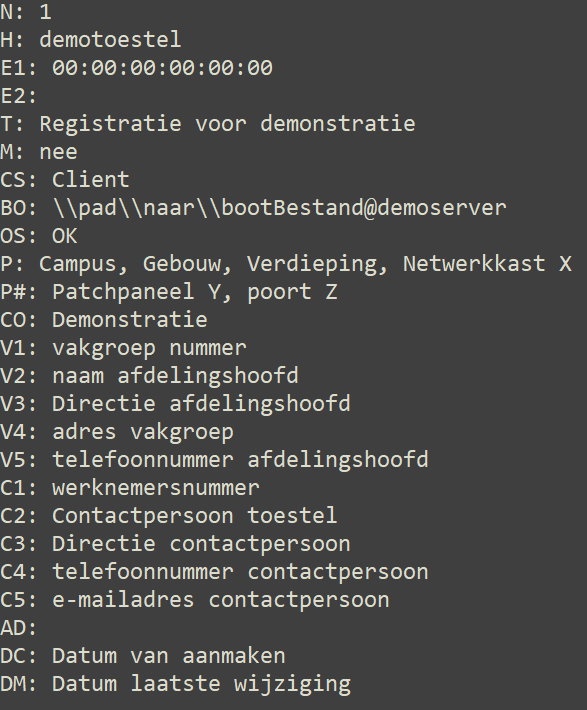
\includegraphics[scale=1.7]{host.png}
%    \caption{host}
%    \label{fig:host}
%\end{figure}
%\begin{figure}[h!]
%    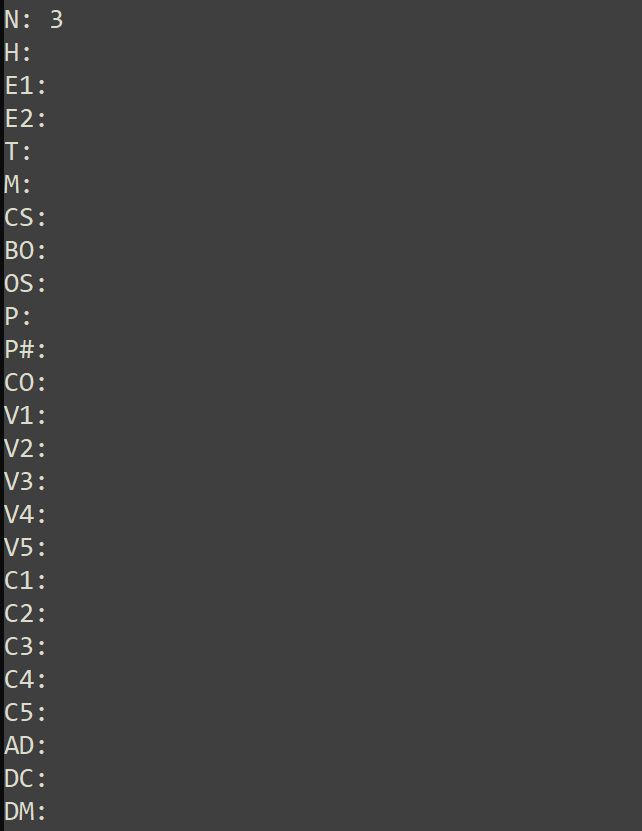
\includegraphics[scale=1.7]{legeHost.png}
%    \caption{lege Host}
%    \label{fig:legeHost}
%\end{figure}

\subsection{Procedure IP registratie voor gebruikers}
\textcolor{purple}{Via de interne webpagina www.netadmin.ugent.be kunnen werknemers van \acrshort{ugent} zowel nieuwe \acrshort{ip} reservaties aanvragen, als bestaande \acrshort{ip} reservaties raadplegen, wijzigen of verwijderen. Bij een nieuwe aanvraag kan men naast de basisinfo, ook de optionele parameters voor een host meegeven zoals beschreven in sectie \ref{subnetbestanden}. Bij wijzigingen kan men alle informatie van de registratie aanpassen, waardoor informatie aan de reservering kan worden toegevoegd, verwijderd of gewijzigd. Het verplaatsen van een host van een subnet naar een ander subnet is eveneens mogelijk door deze vraag mee te sturen naar de netwerkbeheerder via het opmerkingen-veld van de registratie. In figuur \ref{fig:netadmin} zijn de formulieren van deze website weergegeven met data voor demonstratiedoeleinden.
}
\clearpage
\begin{figure*}[h!]
    \centering
    \begin{subfigure}[b]{0.475\textwidth}
        \centering
        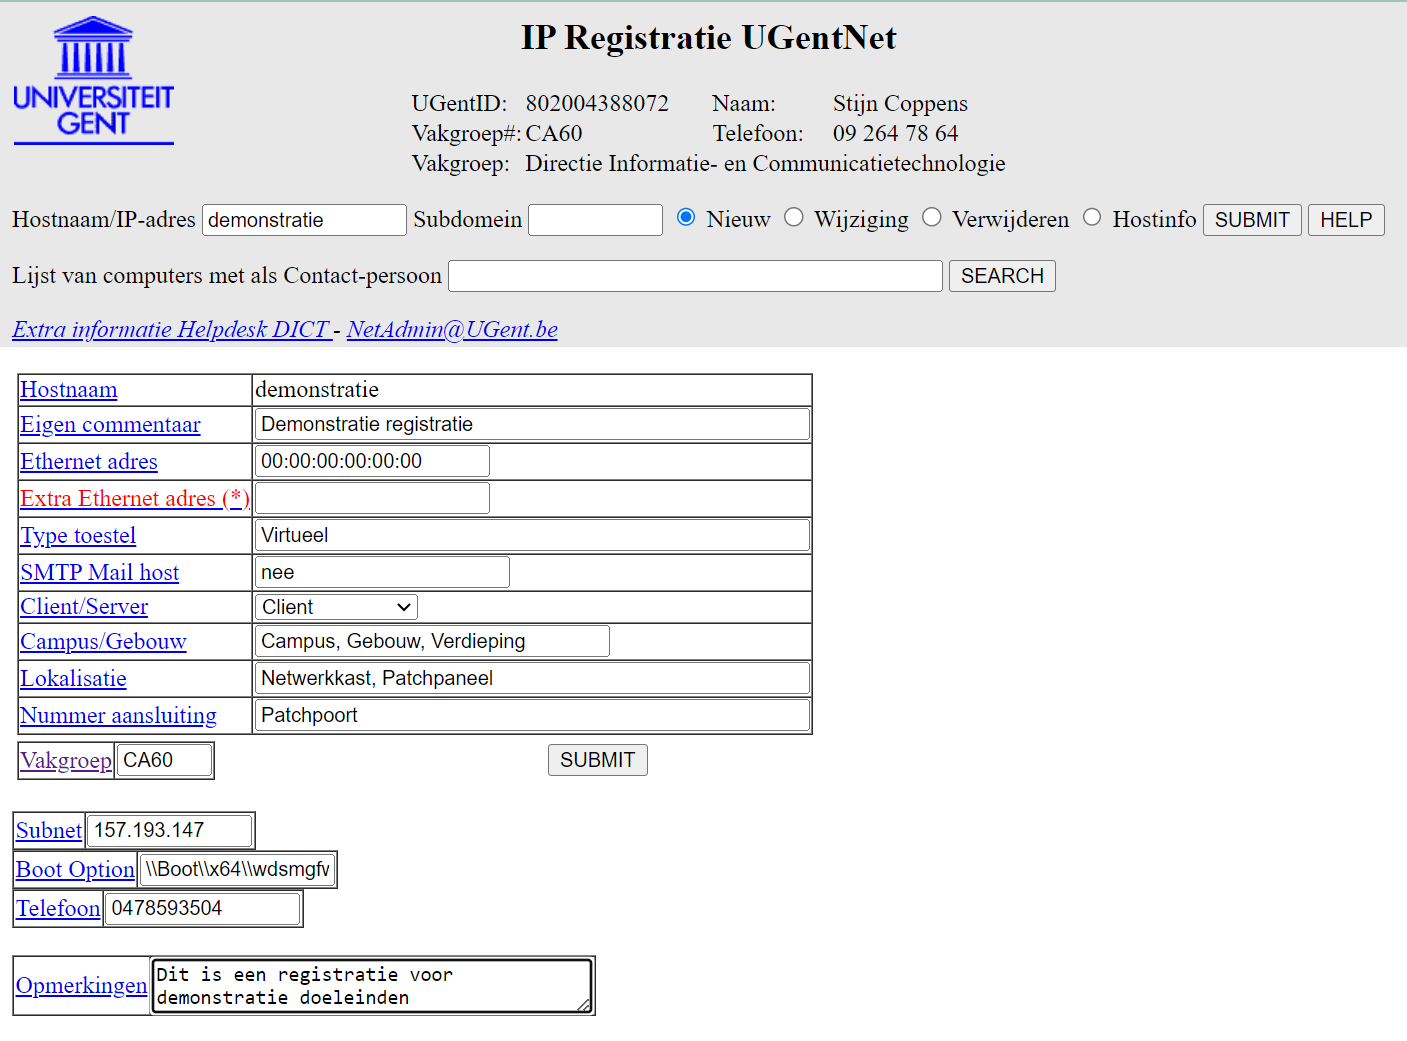
\includegraphics[width=\textwidth]{voorbeeldNieuweRegistratieNetadmin.png}
        \caption{Formulier nieuwe \acrshort{ip}-registratie}
        \label{fig:formNieuwReg}
    \end{subfigure}%
    \hfill
    \begin{subfigure}[b]{0.475\textwidth}
        \centering
        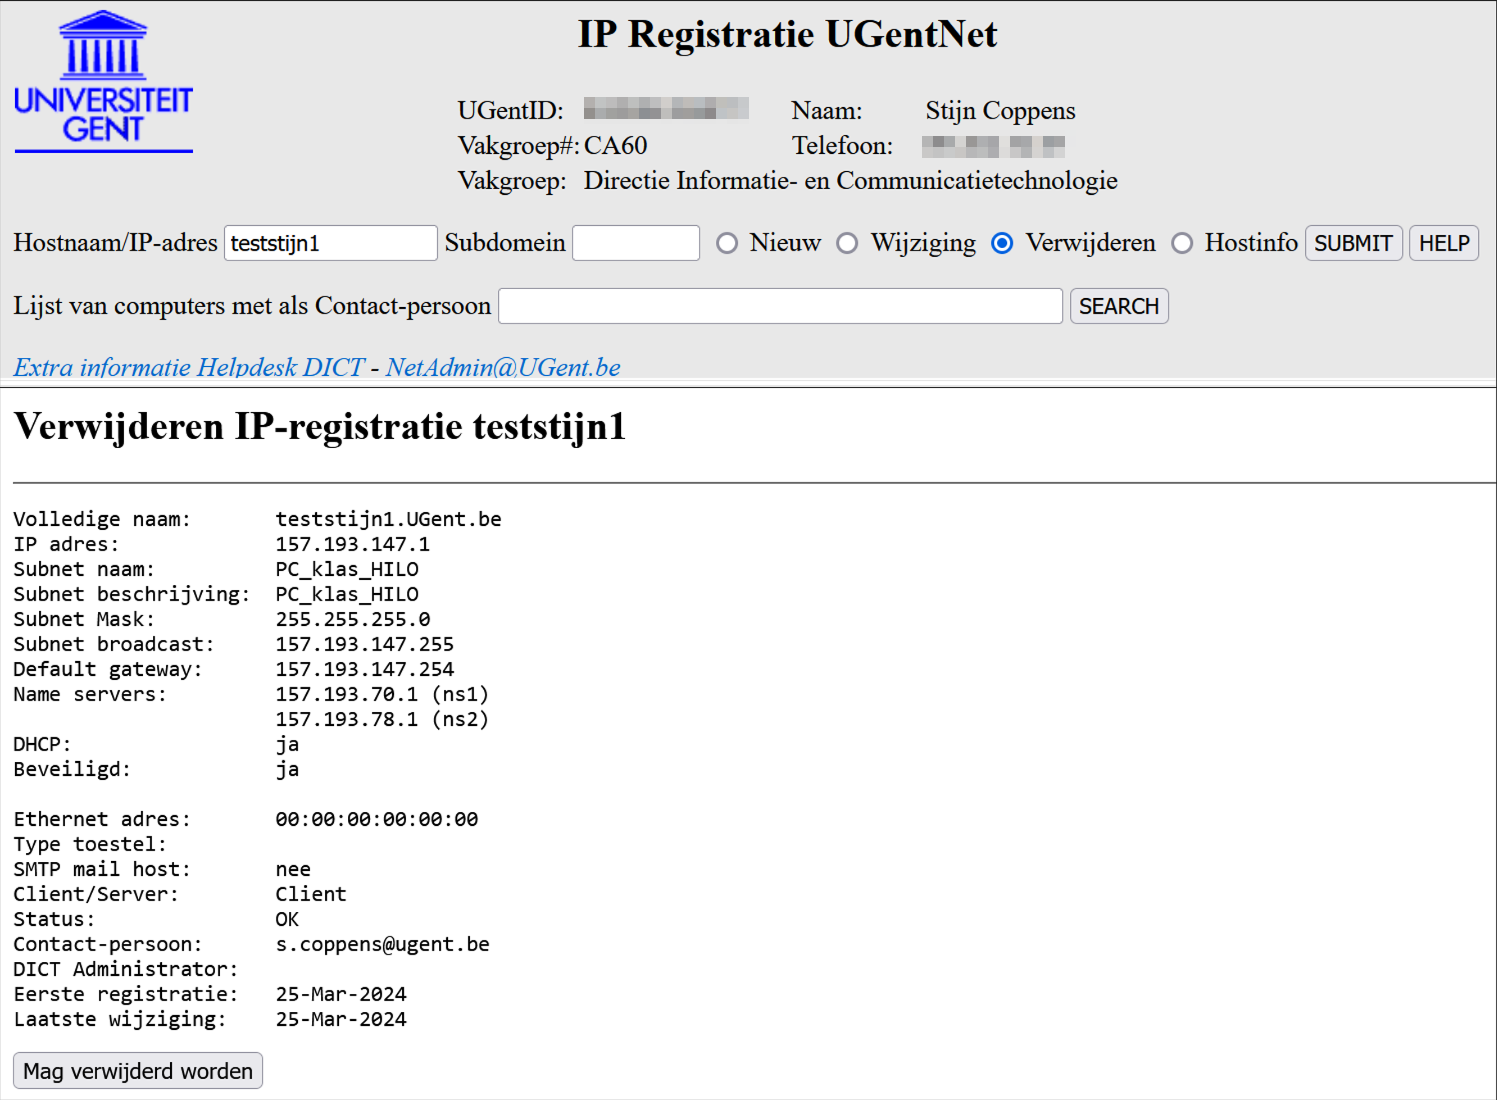
\includegraphics[width=\textwidth]{voorbeeldVerwijderingRegistratieNetadmin.png}
        \caption{Verwijdering \acrshort{ip}-registratie}
        \label{fig:formVerwReg}
    \end{subfigure}
    \vskip\baselineskip
    \begin{subfigure}[b]{0.475\textwidth}
        \centering
        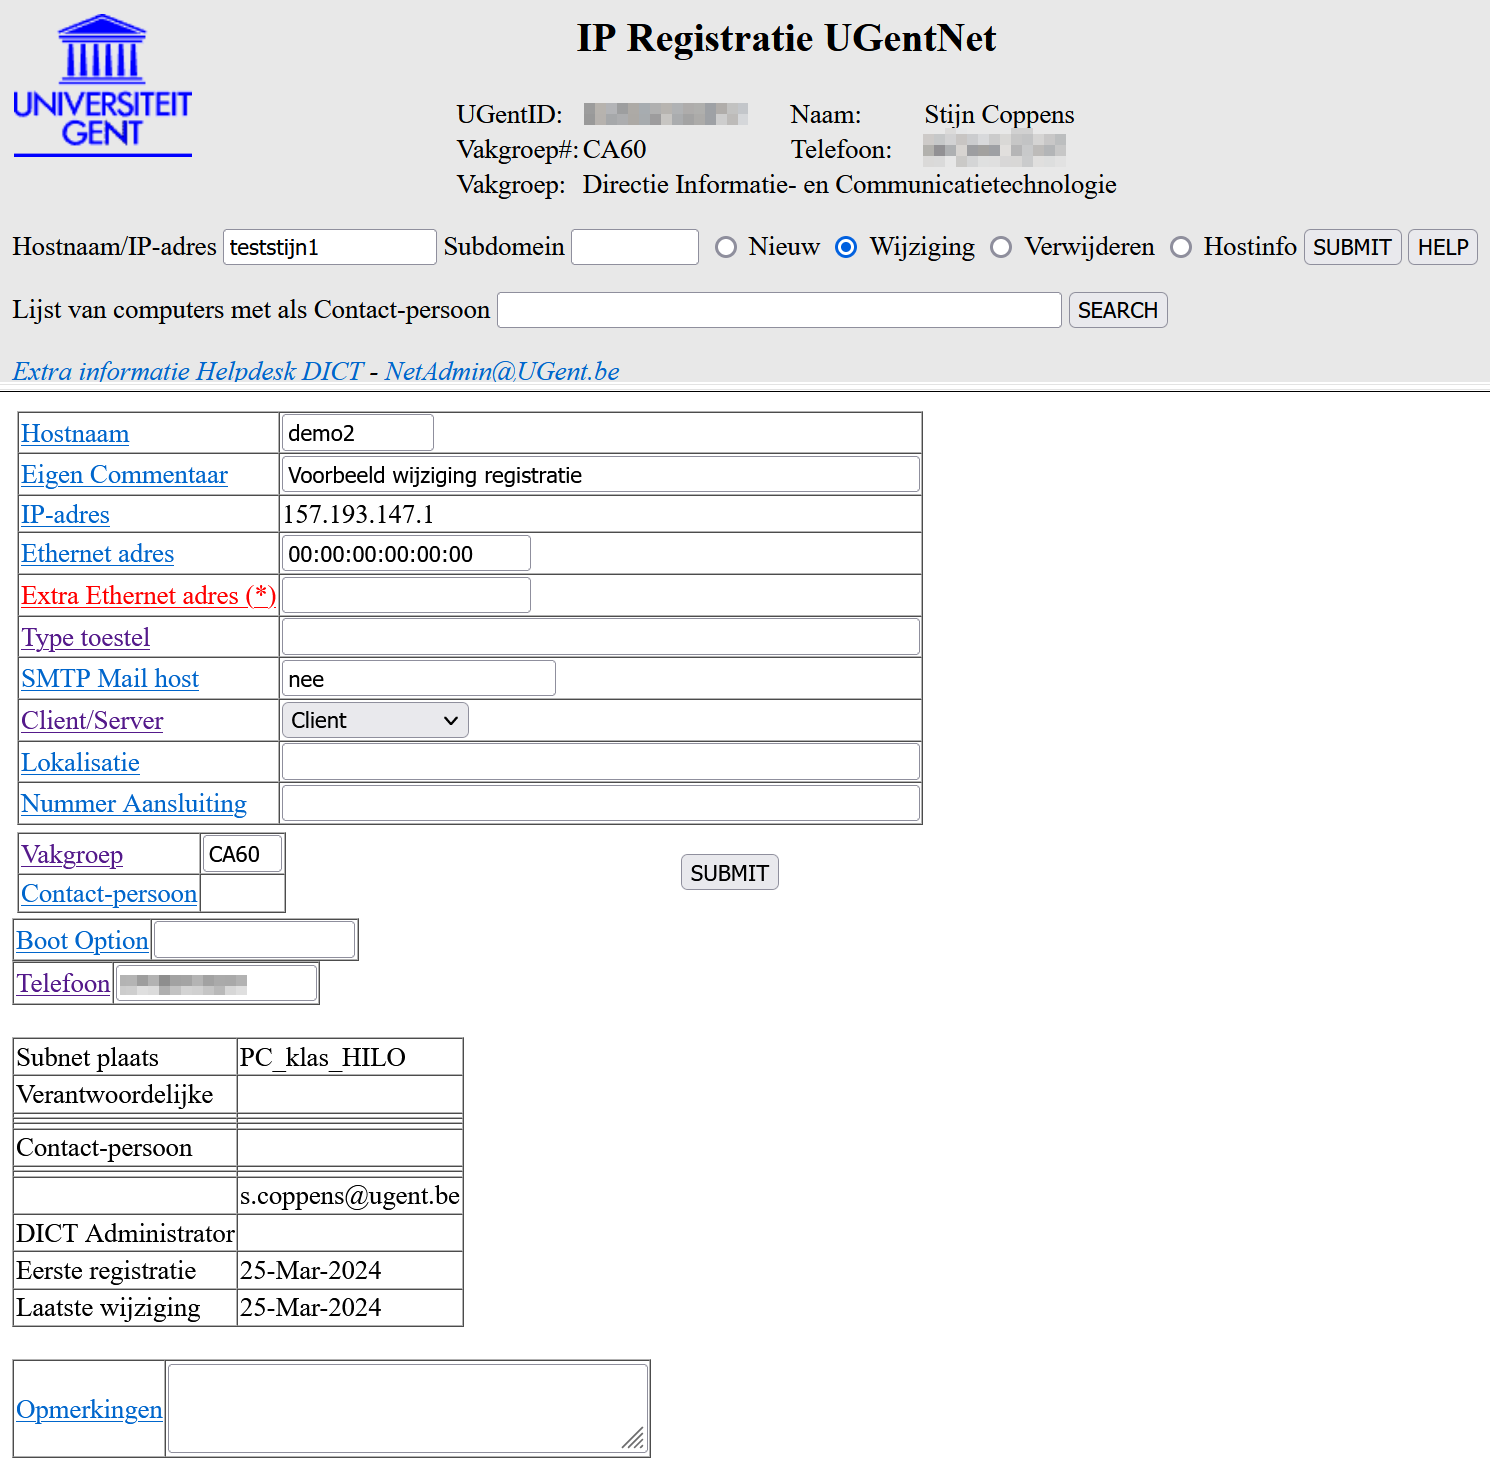
\includegraphics[width=\textwidth]{voorbeeldWijzigingRegistratieNetadmin.png}
        \caption{Formulier wijziging \acrshort{ip}-registratie}
        \label{fig:formWijzReg}
    \end{subfigure}
    \hfill
    \begin{subfigure}[b]{0.475\textwidth}        
        \centering
        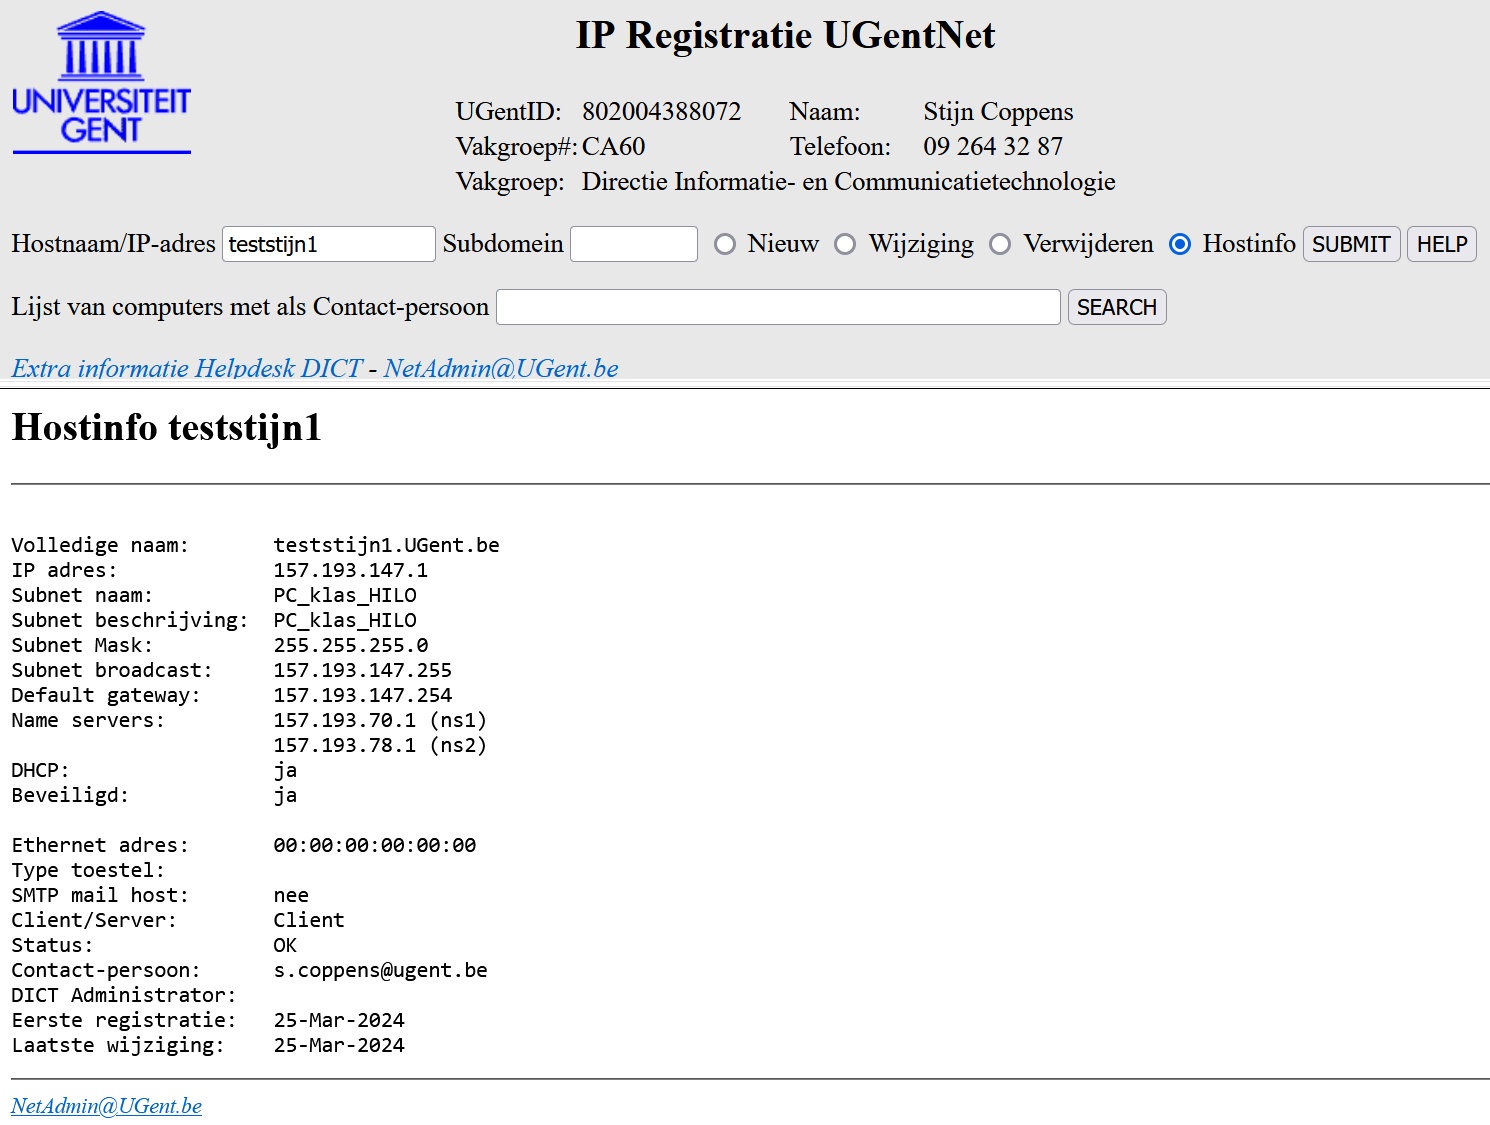
\includegraphics[width=\textwidth]{netadminRaadplegen.png}
        \caption{Raadplegen \acrshort{ip}-registratie}
        \label{fig:raadReg}
    \end{subfigure}    
    \caption{Netadmin website \acrshort{ip}-registratie}
    \label{fig:netadmin}
\end{figure*}


\subsection{Procedure IP registratie voor netwerkbeheerders}
\textcolor{purple}{Nadat de gebruiker op 'submit' klikt zal de \textit{backend} van de website de ingegeven informatie verwerken en als mail verzenden naar de gedeelde mailbox 'netadmin@ugent.be'. Afbeelding \ref{fig:netadminMail} toont drie mails die een netwerkbeheerder dient te behandelen. Elke mail bevat een commando dat de netwerkbeheerder uitvoert op de daarvoor bestemde server in de folder waarin de subnetbestanden staan. Alle informatie in deze afbeeldingen is op basis van de ingegeven informatie in figuren \ref{fig:netadmin}.}
\textcolor{purple}{
    \begin{itemize}
        \item Figuur \ref{fig:nieuwRegMail}: Deze mail geeft alle nodige informatie terug om een nieuwe \acrshort{ip} registratie te maken. Het in de mail beschreven commando \textbf{'mkh B 147 demonstratie'} zal enkele belangrijke taken en controles uitvoeren, waarna de cursor van de beheerder in het eerste vrije adres geplaatst wordt van subnetbestand subnetB147.000. Hierna kan de beheerder alles uit de mail kopiëren beginnende bij \textit{21ddkA} tot en met het einde van de host registratie. Nadat de beheerder het subnetbestand afsluit, zal het script nog enkele controles uitvoeren voor het geval er fouten in de registratie staan. Als de gebruiker in het opmerkingenveld nog informatie heeft geplaatst, zoals netwerkpoorten die open moeten staan, \acrshort{dns} Alias records of andere, dient de netwerkbeheerder dit manueel nog aan te vullen in het subnetbestand.
        \item Figuur \ref{fig:wijzigRegMail}: Deze mail bevat alles voor het wijzigen van een bestaande registratie, het commando in deze mail is \textbf{'chh B 147 teststijn1 demo2'}. Dit proces volgt een vergelijkbare uitvoering als bij het aanmaken van een nieuwe registratie. In dit geval wordt de opgegeven host \textit{teststijn1} gezocht in het subnetbestand subnetB147.000, waarbij de informatie in het subnetbestand wordt overschreven door die van de registratie. Omdat er een tweede hostnaam is opgegeven, zal het commando de hostnaam \textit{teststijn1} ook wijzigen naar de hostnaam \textit{demo2}.
        \item Figuur \ref{fig:verwRegMail}: Deze mail geeft het commando \textbf{'rmhost B 147 teststijn1'}. Dit commando zal, naast enkele controles voor \acrshort{acl}, de host in subnet B 147 opzoeken en vervangen door een lege, vrije host. Dit is het enige commando waarbij de netwerkbeheerder niet in het bestand hoeft te gaan om data te plaatsen, waardoor dit commando ook zeer beperkt is in uitvoeringstijd. Indien de host voorkomt in bepaalde \acrshort{acl}'s kan het zijn dat de netwerkbeheerder eerst de relevante 'S'-lijnen bij andere hosts zal moeten verwijderen waarin deze host voorkomt.
\end{itemize}}

\begin{figure}[H]
    \subfloat[Nieuwe \acrshort{ip} registratie]{%
        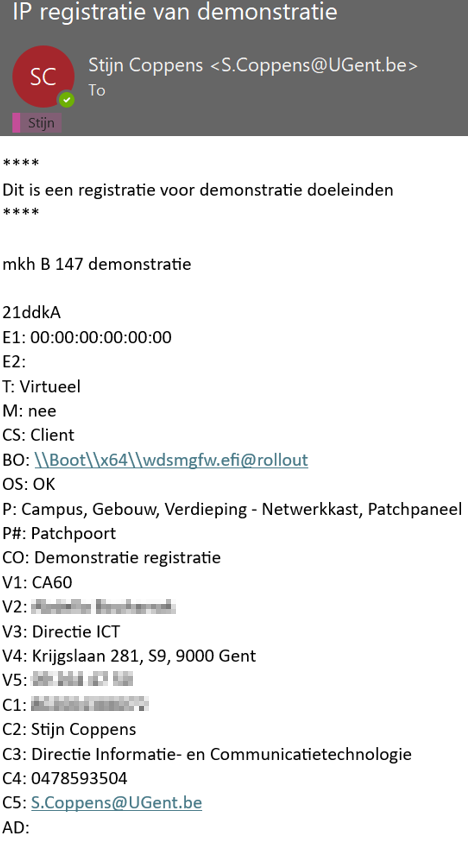
\includegraphics[height=0.4\textheight]{mailNieuweRegistratie.png}
        \label{fig:nieuwRegMail}}
    \hspace*{\fill}
    \subfloat[Wijziging hostnaam \acrshort{ip} registratie]{%
        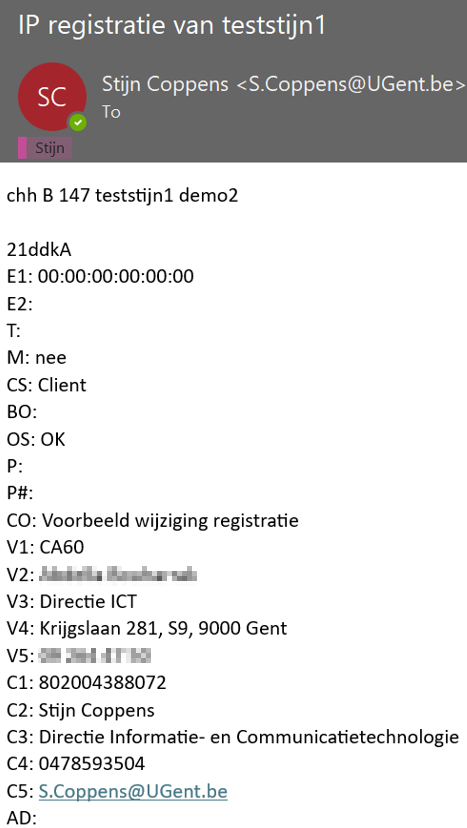
\includegraphics[height=0.4\textheight]{mailWijzigingRegistratie.png}
        \label{fig:wijzigRegMail}}
    \hspace*{\fill}
    \subfloat[Verwijderen \acrshort{ip} registratie]{%
        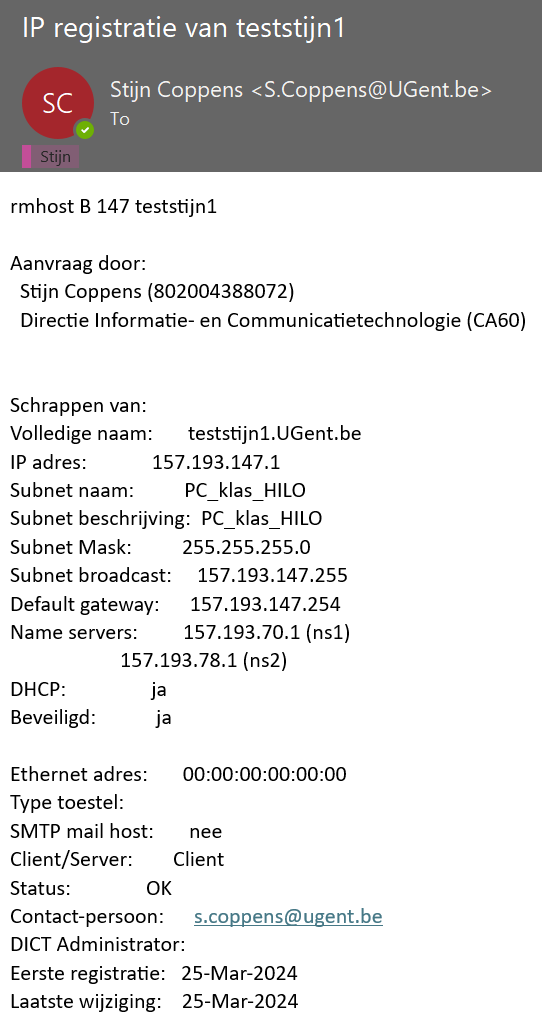
\includegraphics[height=0.4\textheight]{mailVerwijderenRegistratie.png}
        \label{fig:verwRegMail}}
    \caption{Mails \acrshort{ip} Registratie}
    \label{fig:netadminMail}
\end{figure}

\subsection{Aanvullende belangrijke commando's voor subnetbestanden}
\textcolor{purple}{Naast de drie commando's \textbf{'mkh'}, \textbf{'cch'} en \textbf{'rmhost'} voor het verwerken van \acrshort{ip} registraties, zijn er nog enkele andere commando's die relevant zijn te vermelden:}
\textcolor{purple}{
    \begin{itemize}
        \item Hosts verplaatsen: vb. \textbf{'mvh B 147 B 50 teststijn1'} zal een host verplaatsen van subnetbestand subnetB147.000 naar subnetB50.000 
        \item Subnetten opkuisen: vb. \textbf{'unused B 147 400'} geeft alle hosts weer die 400 dagen offline zijn, \textbf{'unused\_rmhost B 147 400'} geeft alle commando's om diezelfde hosts te verwijderen. Om dit werkende te krijgen worden de \acrshort{ARP}-tabellen van alle routers binnen \acrshort{ugent} meerdere keren per dag uitgelezen. Als een toestel verbinding maakt met het netwerk zal het \acrshort{mac}-adres van dit toestel steeds voorkomen in deze tabel. Als het \acrshort{mac}-adres van een host uit subnet B147 dus 400 dagen niet is voorgekomen in een van de \acrshort{arp}-tabellen, dan zal deze weergegeven worden met dit commando.
    \end{itemize}
}

\textcolor{purple}{Het \textbf{'mkh'} commando zal steeds een verwittiging geven als er geen vrije \acrshort{ip}-adressen meer zijn in een subnet. Hier zal de netwerkbeheerder een opkuisactie moeten doen door in te loggen op een andere daarvoor bestemde server, en hier het commando \textbf{'unused B 147 400'} te gebruiken. Dit laatste commando zal alle hosts oplijsten in subnetbestand subnetB147.000 die de laatste 400 dagen niet meer actief geweest zijn op het \acrshort{ugent}-netwerk. Via een pipeline en \textbf{'grep'} kan de netwerkbeheerder de lijst van hosts nog verder filteren op basis van bv. jaartal. Zo krijg je een gelijkaardig commando als \textbf{'unused B 147 400 | grep -v 202[0-4] | grep -v 201[5-9]'}. 
Dit commando zal enkel hosts tonen die de laatste 400 dagen niet online zijn geweest, en waarvan de registratie niet meer werd aangepast sinds 2014. Eens de netwerkbeheerder tevreden is van het aantal hosts die verwijderd zullen worden, kan die het commando nog eens uitvoeren maar dan met \textbf{'unused\_rmhost'} in plaats van \textbf{'unused'}. De output van dit commando zal alle gevraagde 'rmhost' commando's oplijsten die de netwerkbeheerder op de subnetbestanden server kan uitvoeren.}

\textcolor{purple}{Naast deze commando's zijn er ook nog de update-commando's. Pas nadat deze uitgevoerd zijn, zullen alle registraties die gemaakt zijn sinds de vorige uitvoering ook effectief van toepassing zijn. De update-commando's zijn:}
\textcolor{purple}{
    \begin{itemize}
        \item \textbf{'update\_all -load'}: Dit commando zal alle nodige bestanden aanmaken en actief zetten in de \acrshort{dns}-server.
        \item \textbf{'update\_dhcp'}: Dit commando zorgt ervoor dat alle aanpassingen voor \acrshort{dhcp} toegepast worden op de \acrshort{dhcp}-server.
        \item \textbf{'update\_hostlst'}: Dit commando zorgt ervoor dat de hostinfo beschikbaar voor gebruikers op o.a. de netadmin registratie website.
        \item \textbf{'mkacl'}: Dit commando overloopt alle aangemaakt \acrshort{acl}'s.
        \item \textbf{'update\_acl\_write'}: Dit commando zal bij de start van het uitvoeren een wachtwoord opvragen aan de netwerkbeheerder die dit commando ingeeft. Via dit wachtwoord zal dit commando alle \acrshort{acl}-aanpassingen communiceren met de nodige routers.
    \end{itemize}
}
%\begin{figure}[H]
%    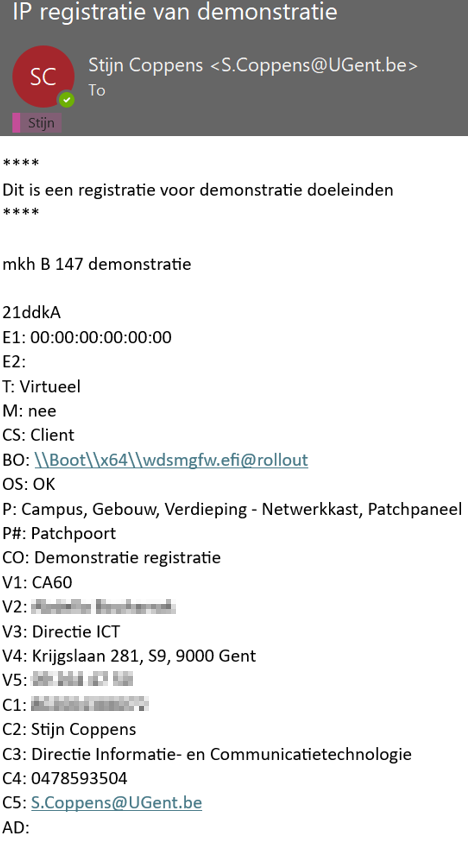
\includegraphics[height=7cm]{mailNieuweRegistratie.png}
%    \caption{Inhoud mail van nieuwe IP-registratie}
%    \label{fig:netadminMail}
%\end{figure}
\textcolor{purple}{
\subsection{Evaluatie subnetbestanden}
Het gebruiken van deze subnetbestanden brengen meerdere uitdagingen met zich mee:
\begin{itemize}
    \item \textbf{Tijd}: Het manueel onderhouden van de scripts, subnetbestanden, netwerkadresreservaties (maken en opkuisen) kan veel tijd vragen. Alle mails met IP registraties moeten elk afzonderlijk bekeken en verwerkt worden.
    \item \textbf{Schaalbaarheid}: Doordat elke wijziging het bestaande bestand overschrijft en er dus geen historische data is kan men moeilijk trends herkennen. Ook wikipediapagina's moet men manueel bijwerken bij grote wijzigingen in de structuur.
    \item \textbf{Consistentie}: De huidige aanpak vraagt meerdere manuele acties, waardoor die vatbaar is voor menselijke fouten of vergissingen. Ook het manueel opzoeken van de relevante subnetbestanden als de aanvrager niet weet in welk subnet de aanvraag terecht moet komen, kan leiden tot registraties in verkeerde subnetten.  
    \item \textbf{Beveiliging}: Zoals beschreven door \textcite{Liao2020} is een van de eerste stappen in een cybersecurity aanval het verzamelen van netwerk informatie via netwerk scan tools zoals 'Nmap'. Het bewaren van alle \acrshort{ip} registraties van het volledige domein centraal in cleartext bestanden, zoals nu het geval is, is dan ook een schat aan informatie voor elke individu met al dan niet slechte bedoelingen.
\end{itemize}
}
\textcolor{purple}{
\section{Status migratie subnetbestanden naar EfficientIP}
Eind 2023 werden de eerste stappen genomen in het project om \acrshort{eip} te implementeren in de werking. Dit project wordt uitgevoerd door Mevr. A. Vandermeeren, vanwege haar uitgebreide kennis van \acrshort{dns} en \acrshort{dhcp} binnen \acrshort{ugent} en Dhr. S. Coppens die de nodige scripts schrijft.
Dit project maakt gebruik van volgende testen, deze worden uitgevoerd zowel bij het implementeren van nieuwe functionaliteiten als bij het testen van scripts.
\begin{itemize}
    \item Manuele \acrshort{eip}-testen: Om na te gaan hoe \acrshort{eip} werkt en hoe bepaalde functionaliteiten reageren op nieuwe informatie worden manuele testen gedaan via de webinterface van \acrshort{eip}.
    \item Postman \acrshort{api}-testen: Via het programma Postman worden manuele testen geschreven die via \acrshort{https} verstuurd worden naar \acrshort{eip}. Dankzij deze testen is er meer inzicht hoe \acrshort{eip} reageert en welke informatie noodzakelijk is.
    \item host- en subnettesten: Om meerdere scenario's te controleren worden in subnetbestand 'subnetB147.000' testen gedaan met het aanmaken, wijzigen en verwijderen van hosts.
\end{itemize}
Sinds de start van het project werden de volgende drie scripts in Python geschreven.
\begin{itemize}
    \item UploadSubnetFile: Dit script maakt via \acrshort{ssh} en \acrshort{scp} een veilige verbinding met de server waarop de subnetbestanden staan en maakt van al deze bestanden een lokale kopie. Hierna doorloopt het script elk bestand, waarop die voor elk bestand de nodige \acrshort{api}-oproepen doet om subnetwerken en hosts aan te maken op \acrshort{eip}.
    \item CreateSubnetFile: Dit script stuurt een \acrshort{api}-oproep naar \acrshort{eip} om alle subnetten op te halen. Hierna haalt het script opnieuw via een \acrshort{api}-oproep voor elk subnet alle hostadressen op. Om dan uiteindelijk lokaal de nodige subnetbestanden aan te maken. Eens al deze subnetbestanden zijn aangemaakt haalt dit script een kopie op van de productie-subnetbestanden, waarop het script voor elk bestand een log wegschrijft met de verschillen tussen het nieuw aangemaakte bestand en het productie-bestand. Tenslotte maakt het script via \acrshort{ssh} en \acrshort{scp} een veilige verbinding met de server waarop de productie-subnetbestanden staan, en plaatst daar zowel de nieuwe subnetbestanden in een tijdelijke folder als alle logs.
    \item CompareAndUpdate: Omdat een referentiepunt nodig is om de aanpassingen te ontdekken in de productie-subnetbestanden, werd op dezelfde server een folder 'LastState' aangemaakt waarin een kopie geplaatst werd van de productiebestanden. Dit script start met via \acrshort{ssh} en \acrshort{scp} een veilige verbinding op te zetten met de server waarop de subnetbestanden staan, waarop die de datum ophaalt van een subnetbestand in de 'LastState'-folder. Hierna zal het script de laatst bewerkte datum van alle productie-subnetbestanden overlopen. Voor elke productie-subnetbestand dat een nieuwere datum heeft, wordt een kopie overgezet van zowel het productie-subnetbestand als de versie in de 'LastState'-folder. Tenslotte worden alle verschillen overlopen en worden de nodige \acrshort{api}-oproepen gedaan om \acrshort{eip} te updaten.
\end{itemize}
}

\section{Volgende stappen in de migratie}
In dit stuk zal ik beschrijven wat de volgende stappen zijn voor de migratie.

% TODO: Beschrijven wat er reeds gedaan is tot nu toe voor de overstap naar EIP
% TODO: Stappen beschrijven hoe we overgaan naar EIP


